\section{Durchführung}
\label{sec:Durchführung}
Grundlegend besteht der Versuchsaufbau aus einem Schwingkreis mit einem Widerstand, einem Kondensator und einer Spule.
    \begin{figure}[H]
        \centering
        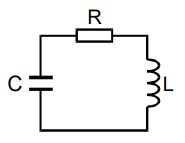
\includegraphics{RLC.PNG}
    \end{figure}
    Der Schwingkreis ist mit einem Frequenzgenerator und einem Oszillographen verbunden.
    Im ersten Teil des Versuchs, der sich mit der Aufgabenstellung a) beschäftigt, wird der Widerstand $R_1 = (30.3 \pm 0.1) \symup{\Omega}$ verwendet; 
    der Kondensator hat eine Kapazität von $C=(5.0 \pm 0.02) \symup{nF}$ und die Induktivität der Spule beträgt $L= (3.5 \pm 0.01)$mH.\\
    Der Frequenzgenerator regt den RLC-Kreis mit einer Rechteckspannung an, die hier $f=242.9$Hz beträgt.\\
    Mit geeigneten Einstellungen am Oszillographen lassen sich so die Amplituden der Schwingung im zeitlichen Verlauf ablesen, woraus anschließend der effektive Dämpfungswiderstand zu bestimmen ist.\\
    Im zweiten Versuchsteil wird dann anstelle von $R_1$ ein variabler Widerstand $R$ verwendet; die vom Generator erzeugte Frequenz ändert sich nicht.\\
    Der Widerstand wird jetzt solange langsam erhöht, bis auf dem Oszillographen keine Schwingung mehr dargestellt wird, sondern der charakteristische Verlauf des aperiodisichen Grenzfalls zu erkennen ist.\\
    Für den letzten Versuchsteil, der die Fragestellungen c) und d) beantworten soll, wird als Widerstand $R_2 = (271.6 \pm 0.2) \symup{\Omega}$ verwendet.
    Außerdem wird der Schwingkreis nun mit einer Sinusfrequenz angeregt. Diese Frequenz wird schrittweise variiert. Auf dem Oszillographen wird neben der Schwingung des RLC-Kreises auch die Frequenz des Generators aufgetragen,
    so dass sich die Phase, die Phasenverschiebung sowie die beiden Amplituden ablesen lassen.
\subsection{Messdaten}
    \begin{figure}[H]
        \hspace*{1cm}
        \begin{minipage}{0.3\textwidth}
        \vspace*{-3.35cm}
        \begin{tabular}{cc}
        \multicolumn{2}{c}{\textbf{Tabelle 1:} Teil a)} \\
        \midrule
        $t[\si{\second}]$ & $U[V]$  \\
        \midrule
        6   &   1.9     \\
        20  &   -1.3    \\
        34  &   0.8     \\
        46  &   -0.65   \\
        62  &   0.35    \\
        76  &   -0.3    \\
        88  &   0.2     \\
        102 &   -0.15   \\
        116 &   0.05    \\
        128 &   -0.1    \\ 
        \end{tabular}
        \end{minipage}
        \begin{minipage}{0.2\textwidth}
        \begin{tabular}{c c c c c}
        \multicolumn{5}{c}{\textbf{Tabelle 2:} Teil c) und d)} \\
        \midrule
        $f[kHZ]$ & $\phi[\mu s]$ & $\increment \phi[\mu s]$ & $A_s[V]$ & $A_g[V]$ \\ 
        \midrule
        5.00   &  200  &  0    &  2.6   &  0.7 \\
        10.00  &  100  &  0    &  2.8   &  0.8 \\
        16.00  &  62   &  0.1  &  3.0   &  0.8 \\
        19.00  &  52   &  2    &  3.2   &  0.1 \\
        21.00  &  48   &  2    &  3.4   &  0.7 \\
        25.00  &  40   &  2    &  4.2   &  0.8 \\
        27.00  &  37   &  3    &  4.8   &  0.8 \\
        30.00  &  33   &  3    &  5.4   &  0.7 \\
        33.00  &  30   &  5    &  6.4   &  0.7 \\
        40.00  &  24   &  8    &  5.6   &  0.7 \\
        43.00  &  24   &  8    &  4.4   &  0.7 \\
        46.00  &  22   &  8    &  3.5   &  0.7 \\
        49.00  &  20   &  9    &  2.8   &  0.7 \\
        52.00  &  19   &  9    &  2.3   &  0.7 \\
        55.00  &  18   &  9    &  1.9   &  0.8 \\
        58.00  &  17   &  8    &  1.6   &  0.8 \\
        60.00  &  16   &  8    &  1.45  &  0.8 \\
        \end{tabular}
        \end{minipage}
    \end{figure}
    \newpage
